\documentclass[a4paper,12pt]{article}
\usepackage{amsmath}
\usepackage{graphicx}
\usepackage{listings}
\usepackage{caption}
\usepackage{hyperref}
\usepackage{booktabs}
\usepackage{pgfplots} % For including plots
\usepackage{ragged2e}
\usepackage{listings}
\usepackage{float}
\usepackage{geometry}
\geometry{margin=2.5cm} % <-- Set all margins to 2.5cm. Change as needed.
\usepackage[most]{tcolorbox}

\hypersetup{
    hidelinks
}


\usepackage{xcolor}

\definecolor{codegreen}{rgb}{0,0.6,0}
\definecolor{codegray}{rgb}{0.5,0.5,0.5}
\definecolor{codepurple}{rgb}{0.58,0,0.82}
\definecolor{backcolour}{rgb}{0.95,0.95,0.92}

\tcbset{
    frame code={},
    center title,
    left=0pt,
    right=0pt,
    top=0pt,
    bottom=0pt,
    colback=backcolour,
    colframe=white,
    width=\dimexpr\textwidth\relax,
    enlarge left by=0mm,
    boxsep=5pt,
    arc=0pt,outer arc=0pt,
    }



\lstdefinestyle{mystyle}{
    backgroundcolor=\color{backcolour},   
    commentstyle=\color{codegreen},
    keywordstyle=\color{magenta},
    numberstyle=\tiny\color{codegray},
    stringstyle=\color{codepurple},
    basicstyle=\ttfamily\footnotesize,
    breakatwhitespace=false,         
    breaklines=true,                 
    captionpos=b,                    
    keepspaces=true,                 
    numbers=left,                    
    numbersep=5pt,                  
    showspaces=false,                
    showstringspaces=false,
    showtabs=false,                  
    tabsize=2
}

\lstset{style=mystyle}
% \documentclass{article}
\usepackage{graphicx} % Required for inserting images

\title{Human Computer Interaction}
\author{Budgify Report}
\date{Authors:\\ Onorio Iacobelli\\Alessandro Rocchi\\Alessandro Catalano}

\begin{document}

\maketitle

\tableofcontents

\section{Introduction}
Our idea was to create an application that would help users in managing their finances and set new goals. We didn't focus on a specific target audience as this is a topic relevant for all people, no matter age or job.

\section{Requirements Analysis}

\subsection{Personas and Scenarios}

\subsubsection{Alex Jameson – The Student with the Dream of a Car}
\begin{enumerate}
    \item Personality and Behavior:
    
    Alex is an ambitious and forward-thinking university student, constantly striving for independence. He's disciplined in his studies and works part-time, but struggles with self-control when it comes to impulsive spending. Deep down, Alex is motivated by the desire to prove to himself and others that he can achieve major life goals on his own. He values freedom and sees owning a car as a symbol of personal success and responsibility.
    
    \item Scenario:
    
    Alex dreams of buying his first car but feels overwhelmed trying to balance his school workload, part-time job, and unpredictable spending habits. When he starts using "Budgify", it becomes more than just a budgeting tool, it’s his personal financial coach.
    
    \item Impact of "Budgify":
    
    Goal-Oriented Mindset: Alex sets a specific savings goal in "Budgify" for his car, breaking it down into manageable monthly targets. Seeing his progress visually keeps him motivated and focused.
    
    Behavioral Awareness: With "Budgify" spending insights, Alex becomes more aware of his habitual takeout expenses. Recognizing the impact, he starts meal-prepping, not only saving money but also improving his health and self-discipline.
    
    Thanks to "Budgify", Alex gains a stronger sense of control and confidence in his financial decisions, ultimately purchasing his car without compromising his long-term security.

\end{enumerate}
\subsubsection{James Carter – The Man Who Got Fired}
\begin{enumerate}
    \item Personality and Behavior:
    
    James is a practical and resilient individual in his late 30s who thrives on stability. When he loses his job, his initial reaction is anxiety, bordering on hopelessness. Internally, he struggles with self-worth and the fear of losing control. However, James is also adaptive and willing to rebuild. He's detail-oriented and appreciates clarity when faced with uncertainty.
    
    \item Scenario:
    After being unexpectedly laid off, James feels lost and unsure of how long he can stay afloat. He turns to "Budgify" to regain a sense of direction and clarity during this uncertain time.
    
    \item Impact of "Budgify":
    
    Clarity in Chaos: "Budgify" helps James analyze his emergency fund and sets a realistic timeline for how long his current savings will last. This calms his anxiety and lets him focus strategically on his next steps.
    
    Structured Transition: As he begins freelancing, James uses "Budgify" to categorize different income sources, track tax-related expenses, and manage invoices. This organization helps him treat freelancing as a viable and structured career path.
    
    Thanks to "Budgify", James rebuilds his confidence and navigates unemployment with purpose, eventually stabilizing his finances and redefining his professional future.

\end{enumerate}
\subsubsection{Margaret "Maggie" Thompson – The Elder Who Wants to Go on a Cruise}
\begin{enumerate}
    \item Personality and Behavior:
    
    Maggie is a lively, optimistic retiree with a zest for life. She’s careful with money but believes in enjoying the fruits of her lifelong labor. Internally, she’s driven by the need to feel independent and self-sufficient, even in her golden years. She's curious, enjoys planning, and takes pride in managing her finances herself rather than relying on her children.
    
    \item Scenario:
    
    With a long-anticipated cruise around the Mediterranean on the horizon, Maggie wants to enjoy herself without falling into careless spending. She downloads "Budgify" to help her prepare for the trip.
    
    \item Impact of "Budgify":
    
    Confident Planning: Maggie uses "Budgify" to create a personalized trip budget, dividing expenses into categories like travel, lodging, excursions, and on-board spending. The app gives her peace of mind by projecting her affordability.
    
    Conscious Spending: During the trip, "Budgify" tracks her spending in real time, sending gentle alerts when she’s nearing her limits. This empowers her to make informed choices—buying meaningful souvenirs while skipping unnecessary extras.
    
    Thanks to "Budgify", Maggie enjoys her cruise worry-free, proud of having full control over her finances, and returns home with wonderful memories—not debt.
\end{enumerate}
\subsection{User analysis}

\subsubsection{Questionnaire}

\begin{figure}[H]
    \centering
    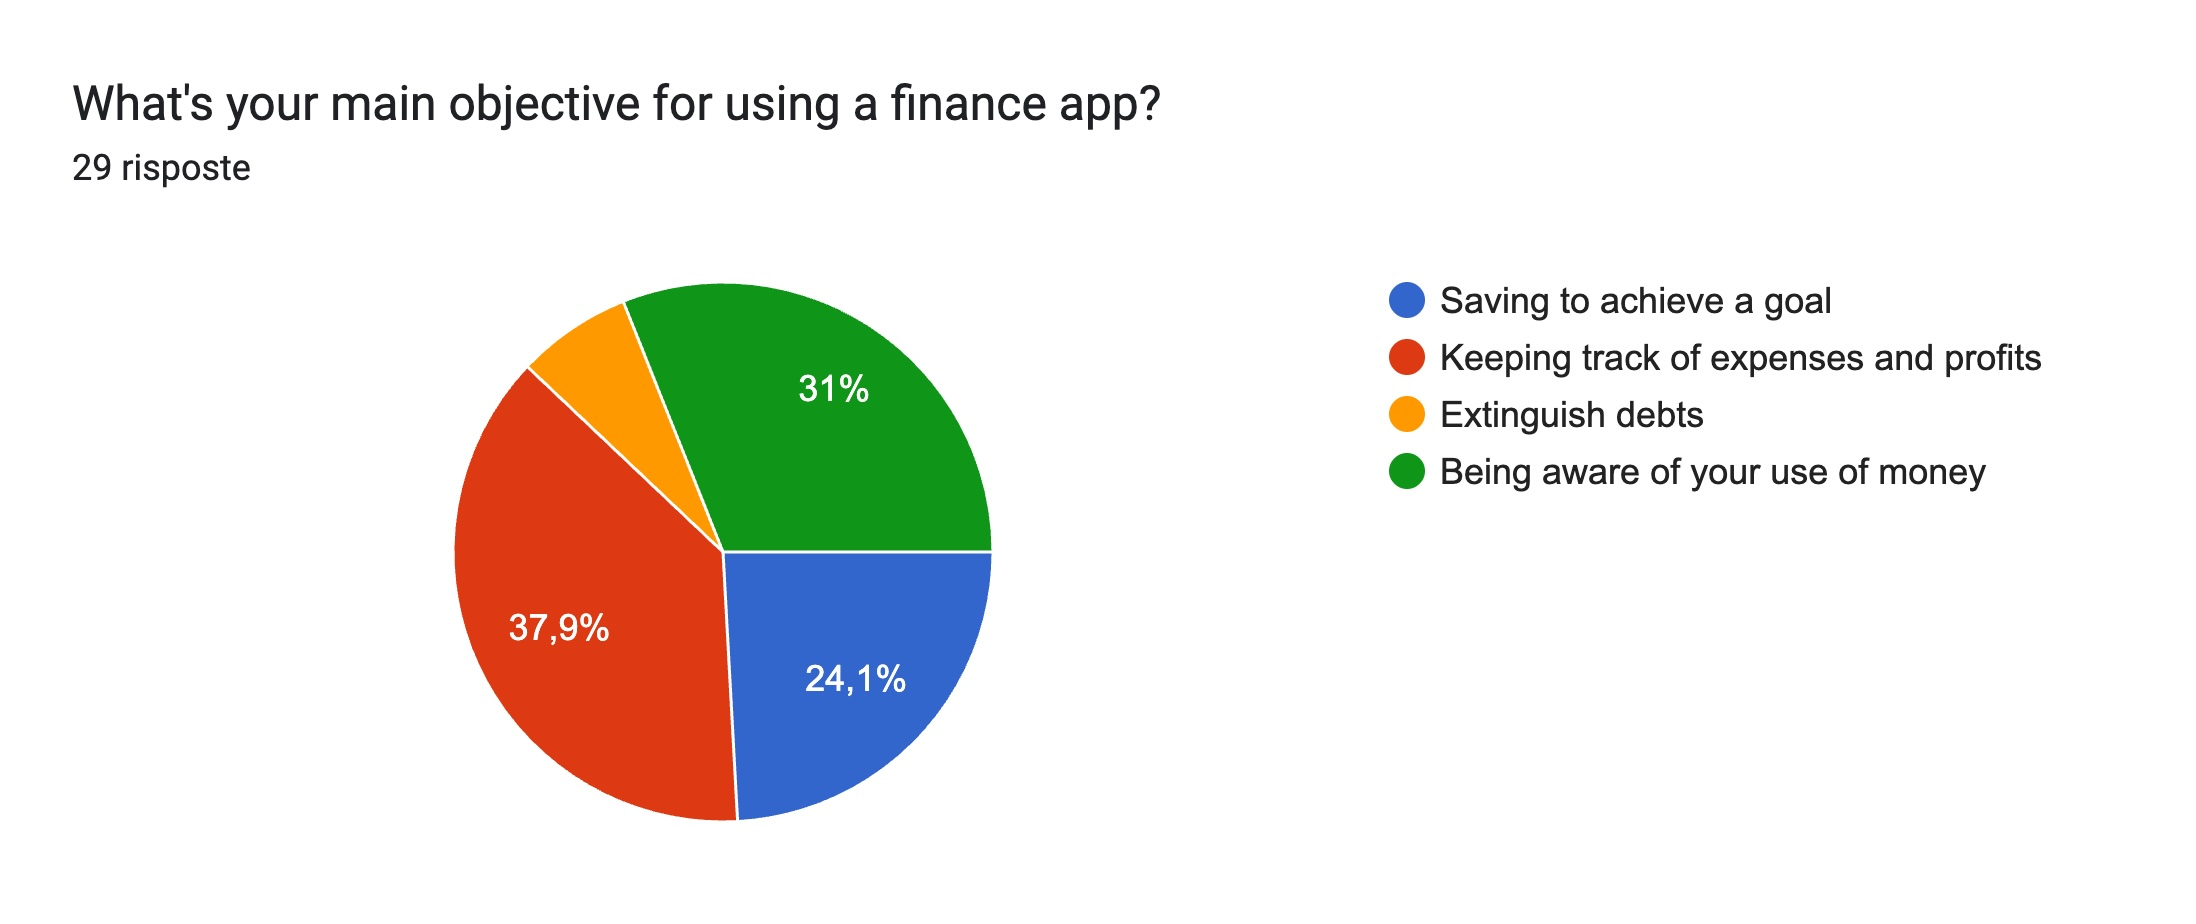
\includegraphics[width=\linewidth]{imagequest1.jpg}
\end{figure}

\begin{figure}[H]
    \centering
    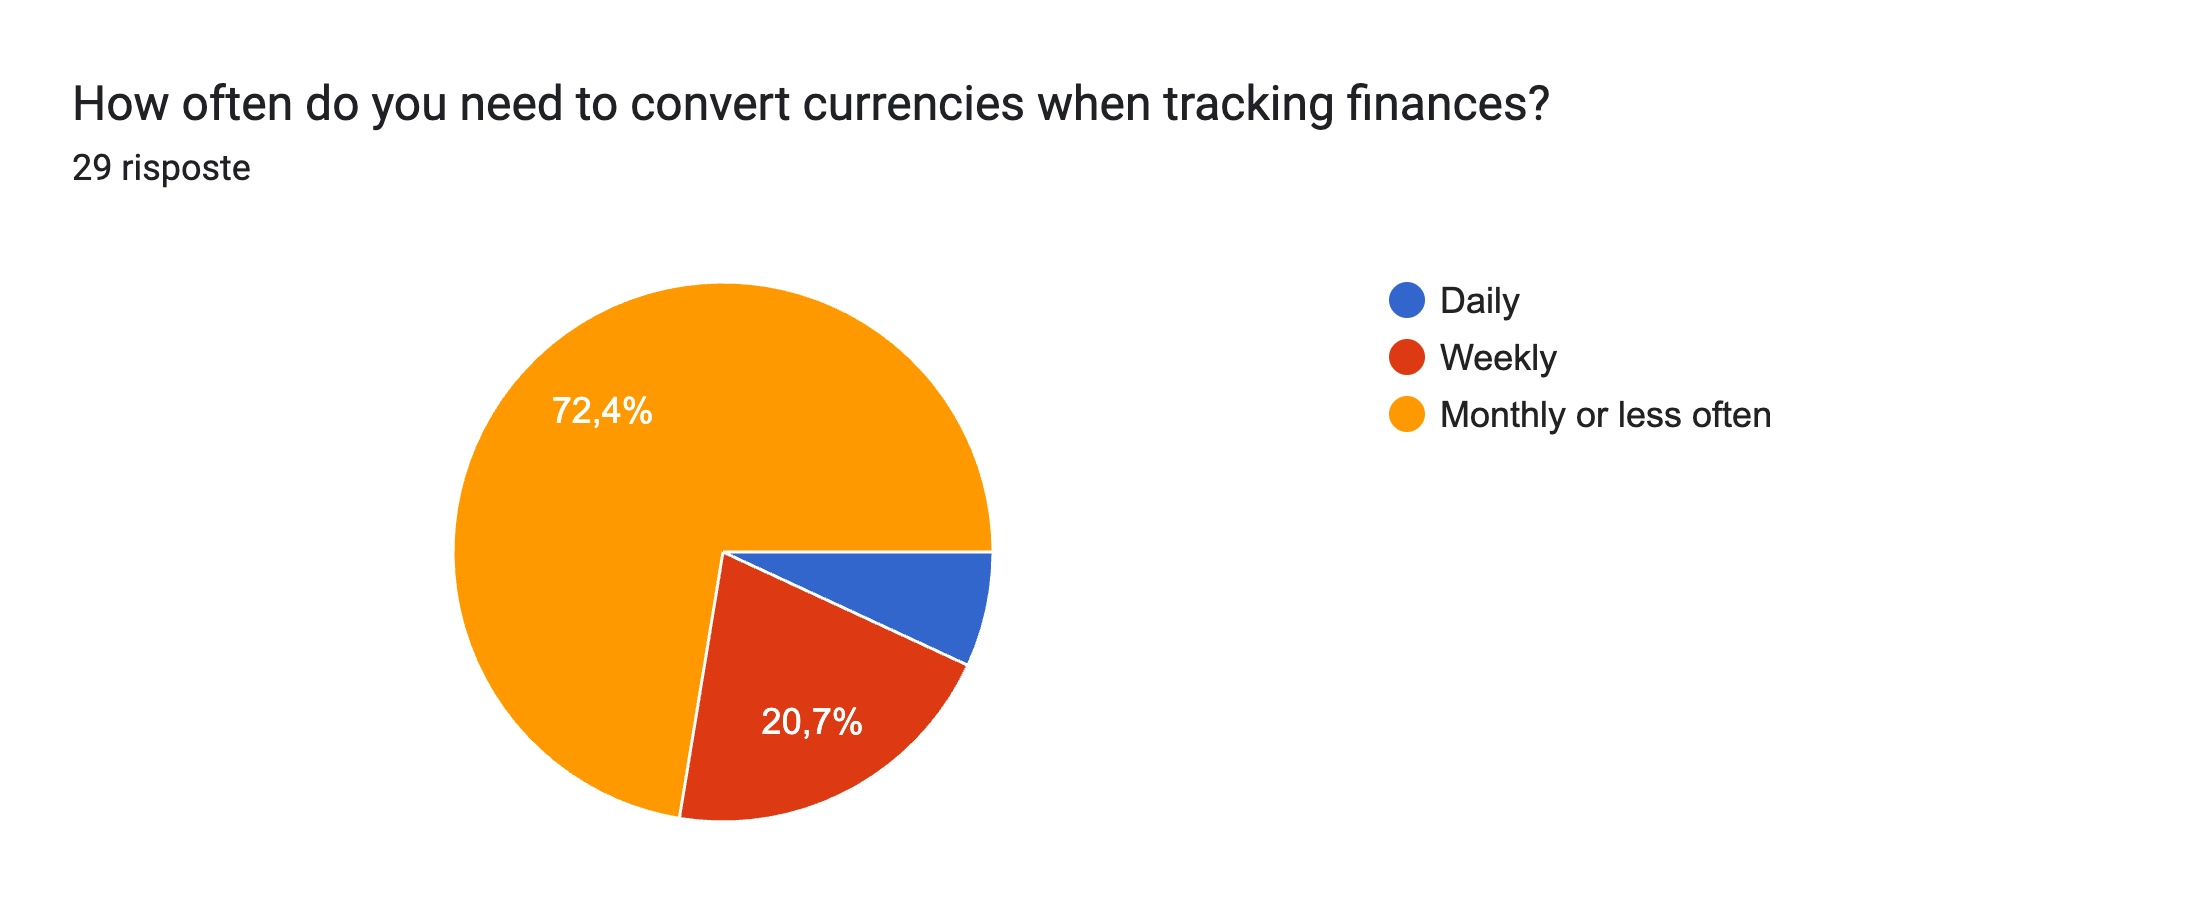
\includegraphics[width=\linewidth]{imagequest2.jpg}
\end{figure}

\begin{figure}[H]
    \centering
    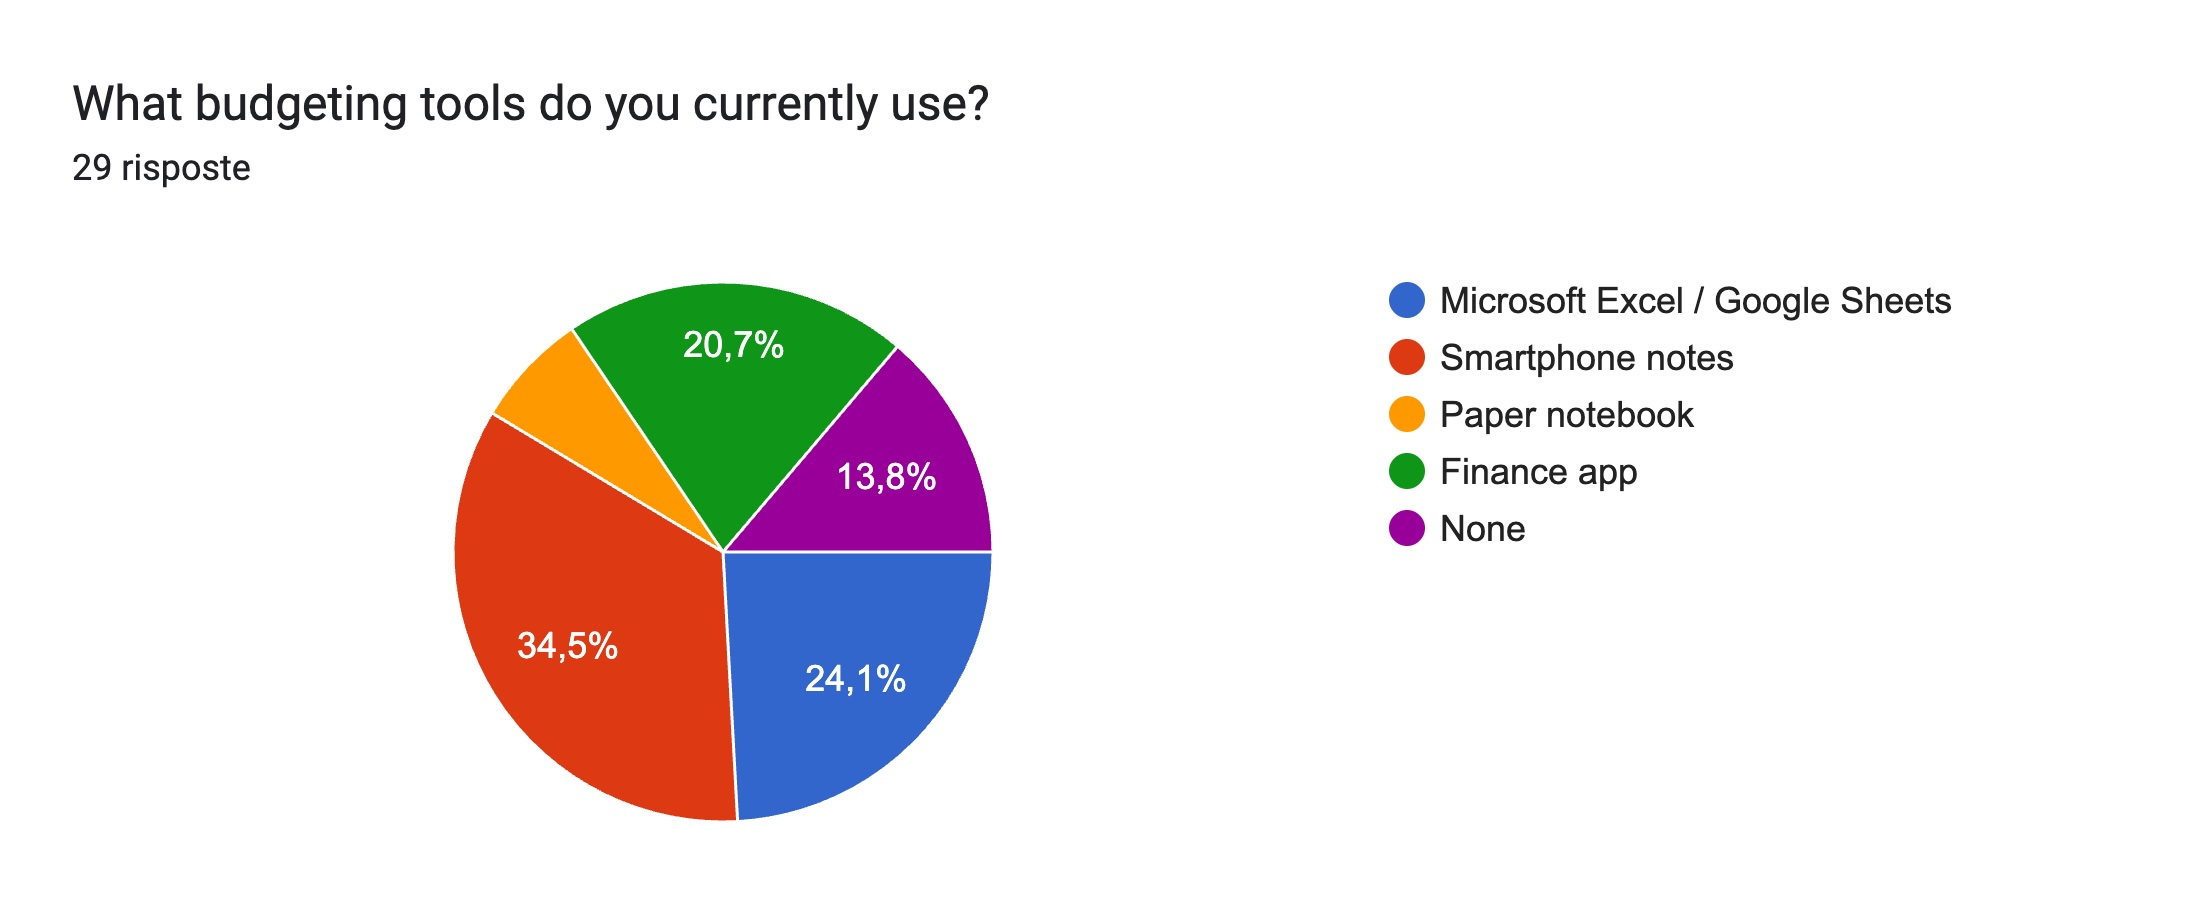
\includegraphics[width=\linewidth]{imagequest3.jpg}
\end{figure}

\begin{figure}[H]
    \centering
    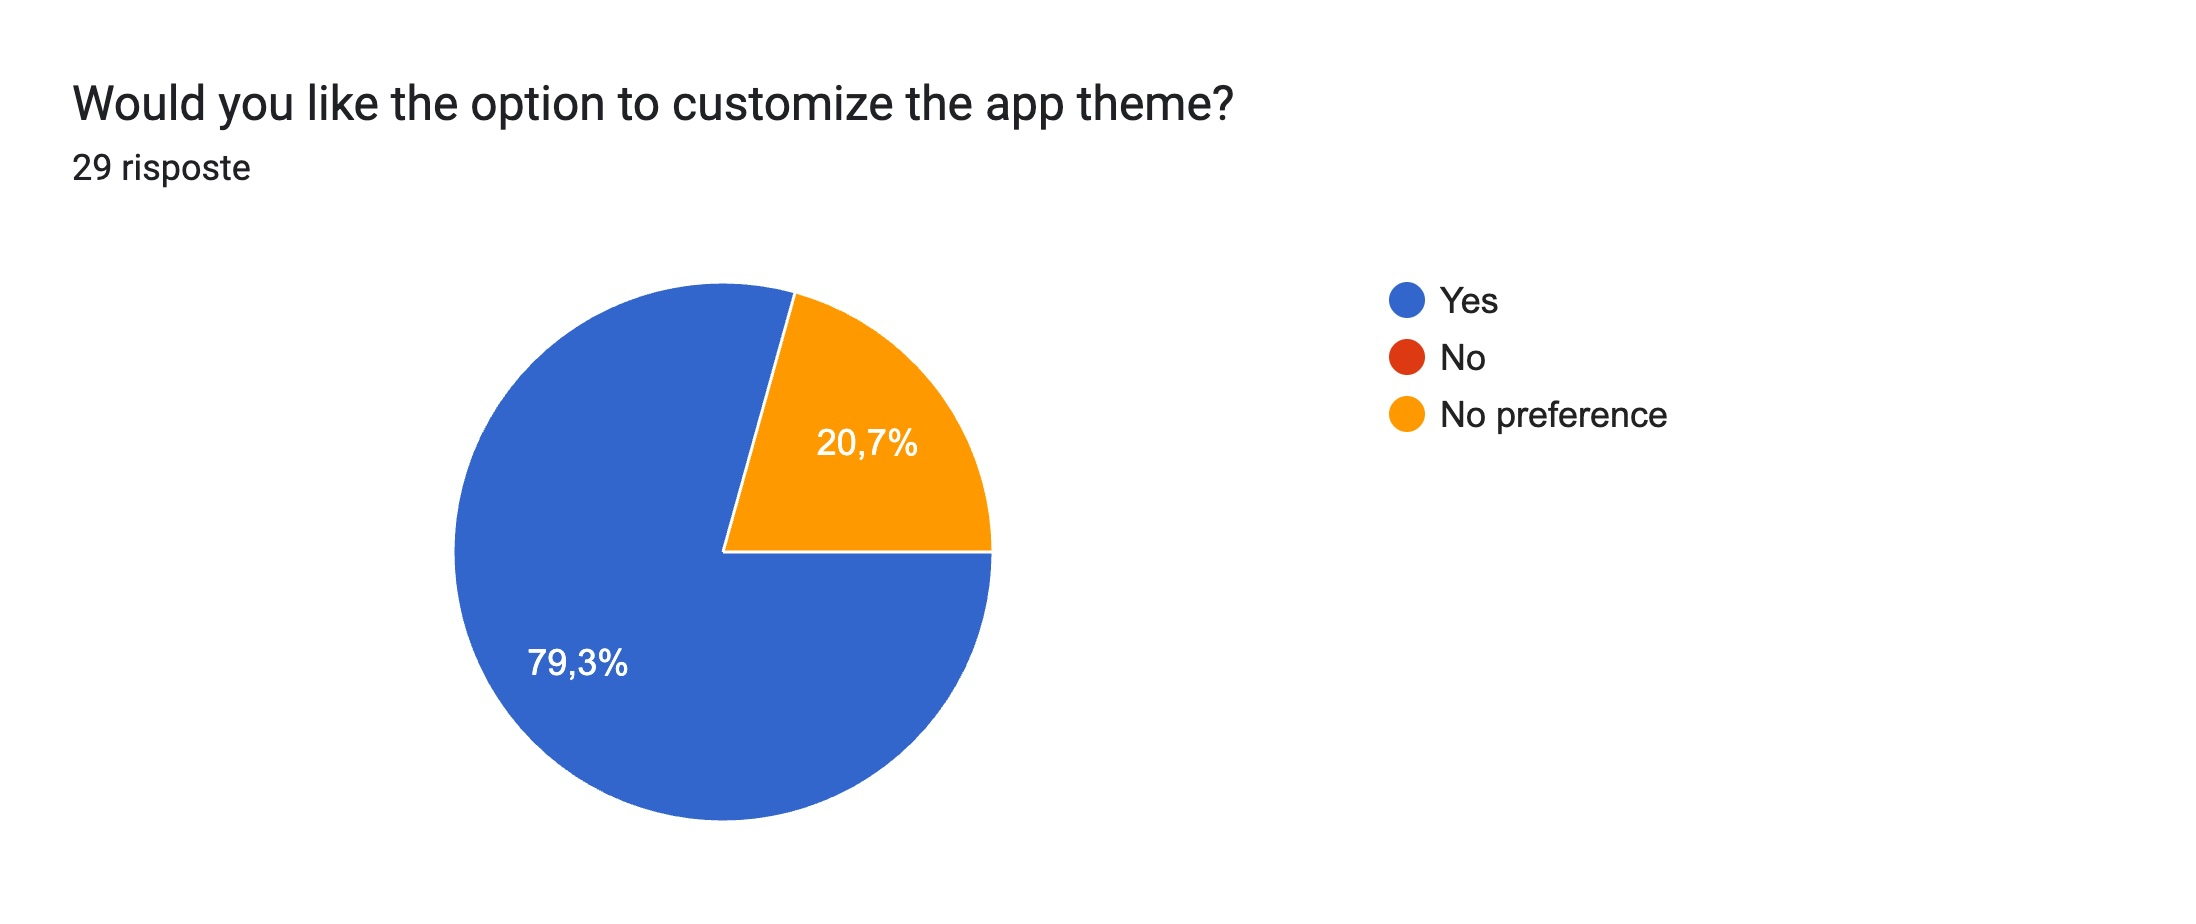
\includegraphics[width=\linewidth]{imagequest4.jpg}
\end{figure}

\begin{figure}[H]
    \centering
    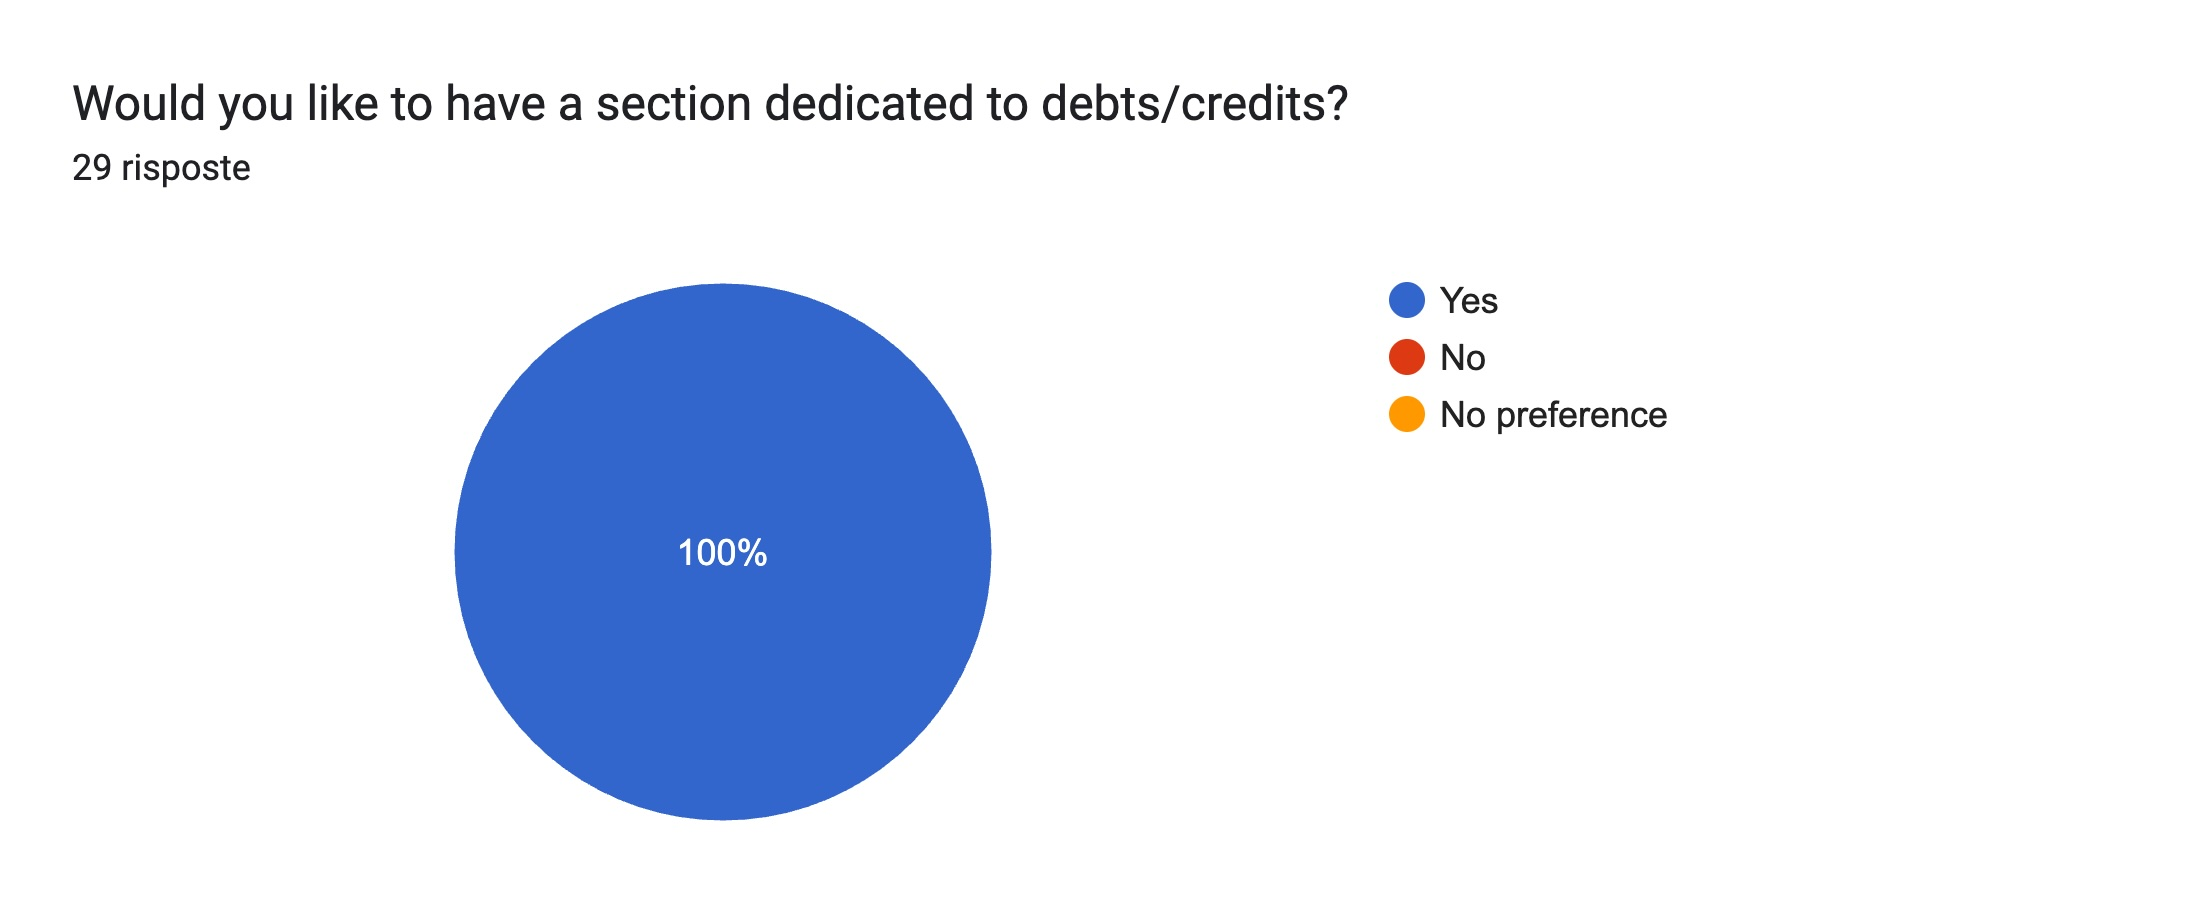
\includegraphics[width=\linewidth]{imagequest5.jpg}
\end{figure}

\begin{figure}[H]
    \centering
    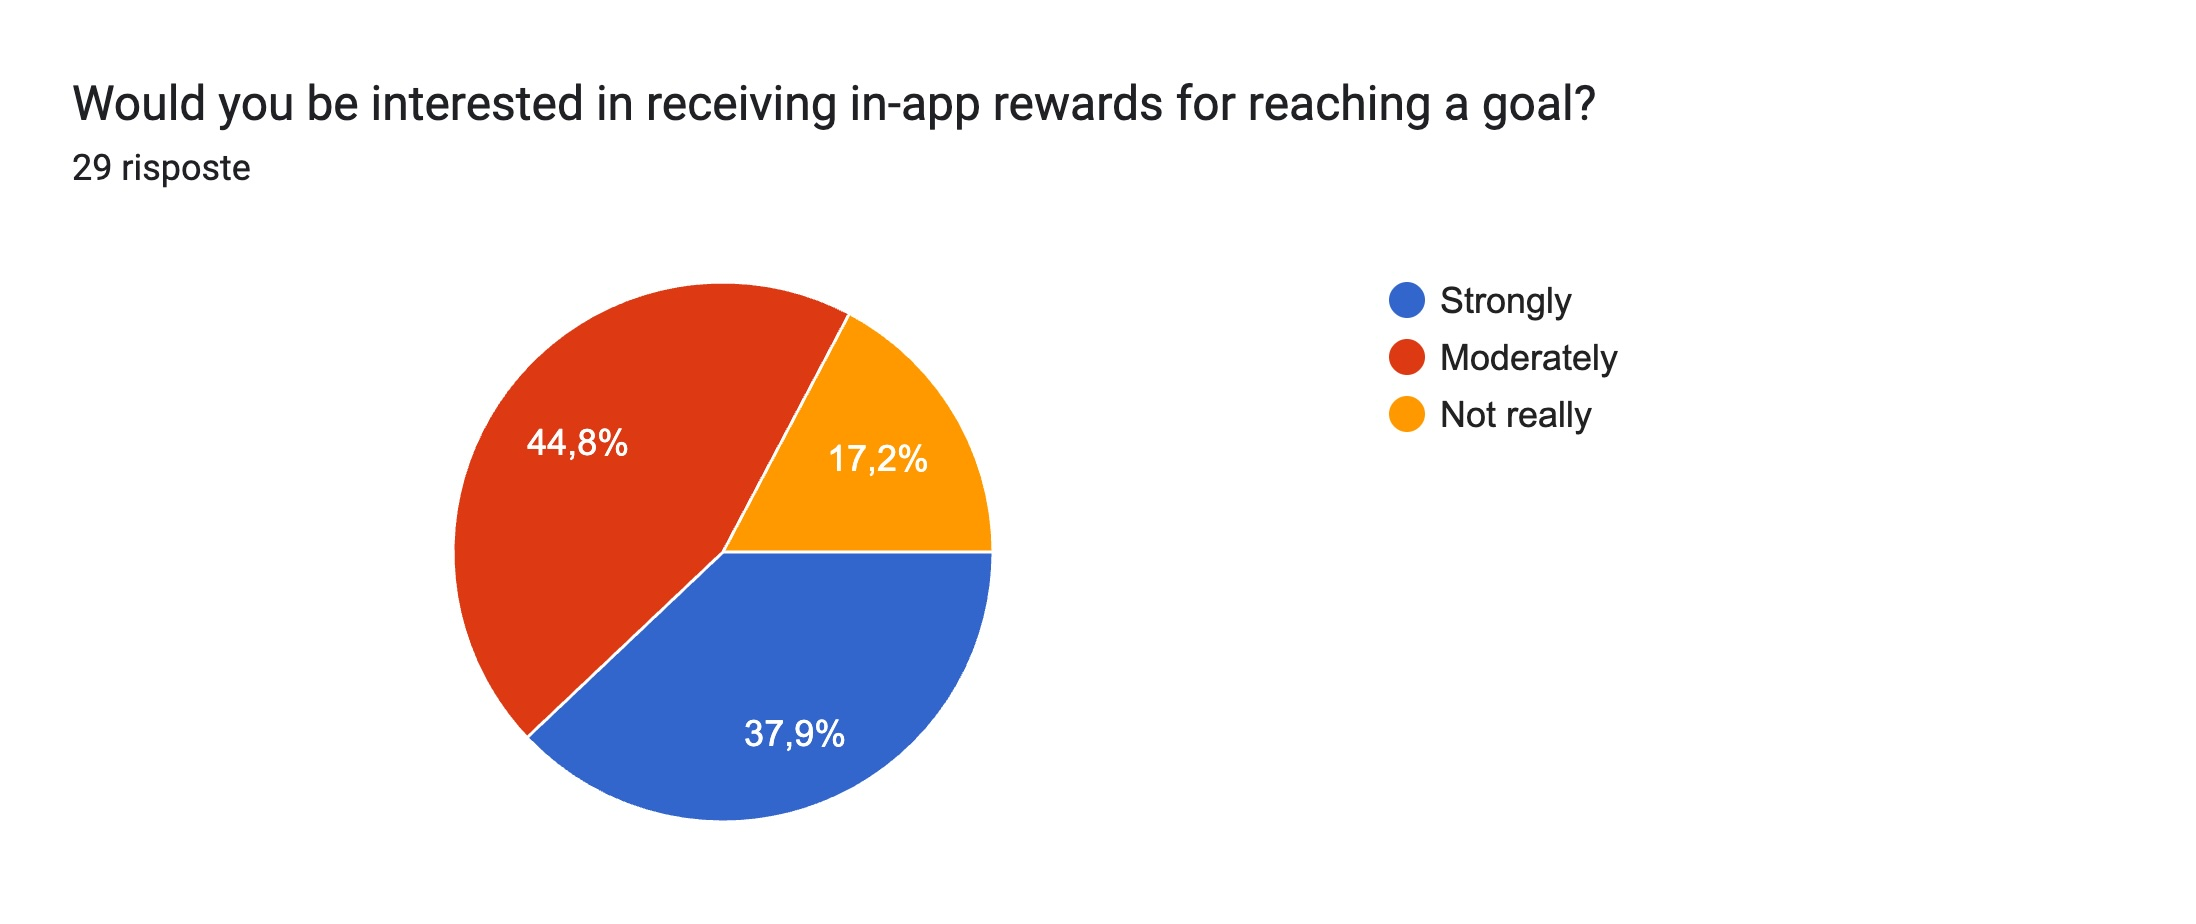
\includegraphics[width=\linewidth]{imagequest6.jpg}
\end{figure}

\begin{figure}[H]
    \centering
    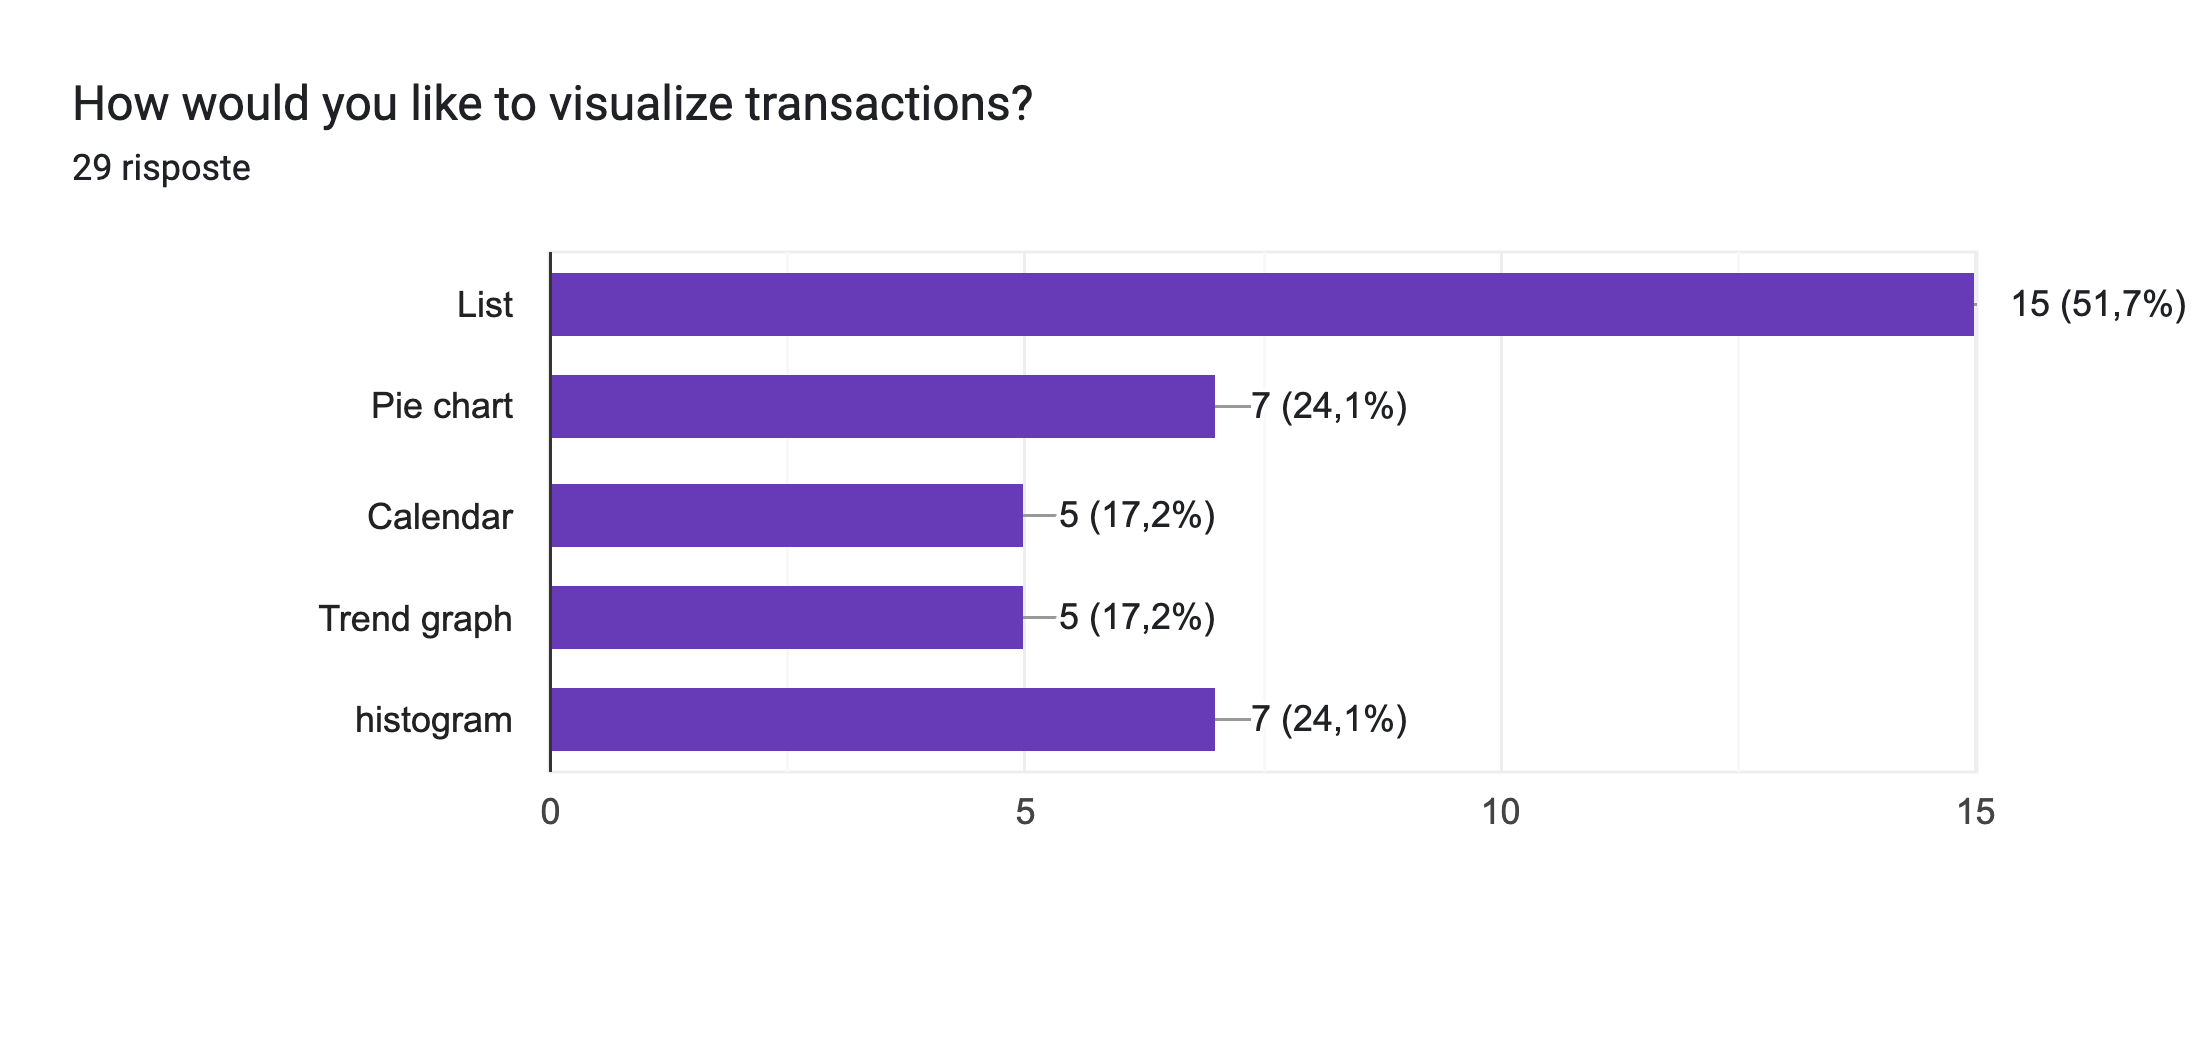
\includegraphics[width=\linewidth]{imagequest7.jpg}
\end{figure}

\begin{figure}[H]
    \centering
    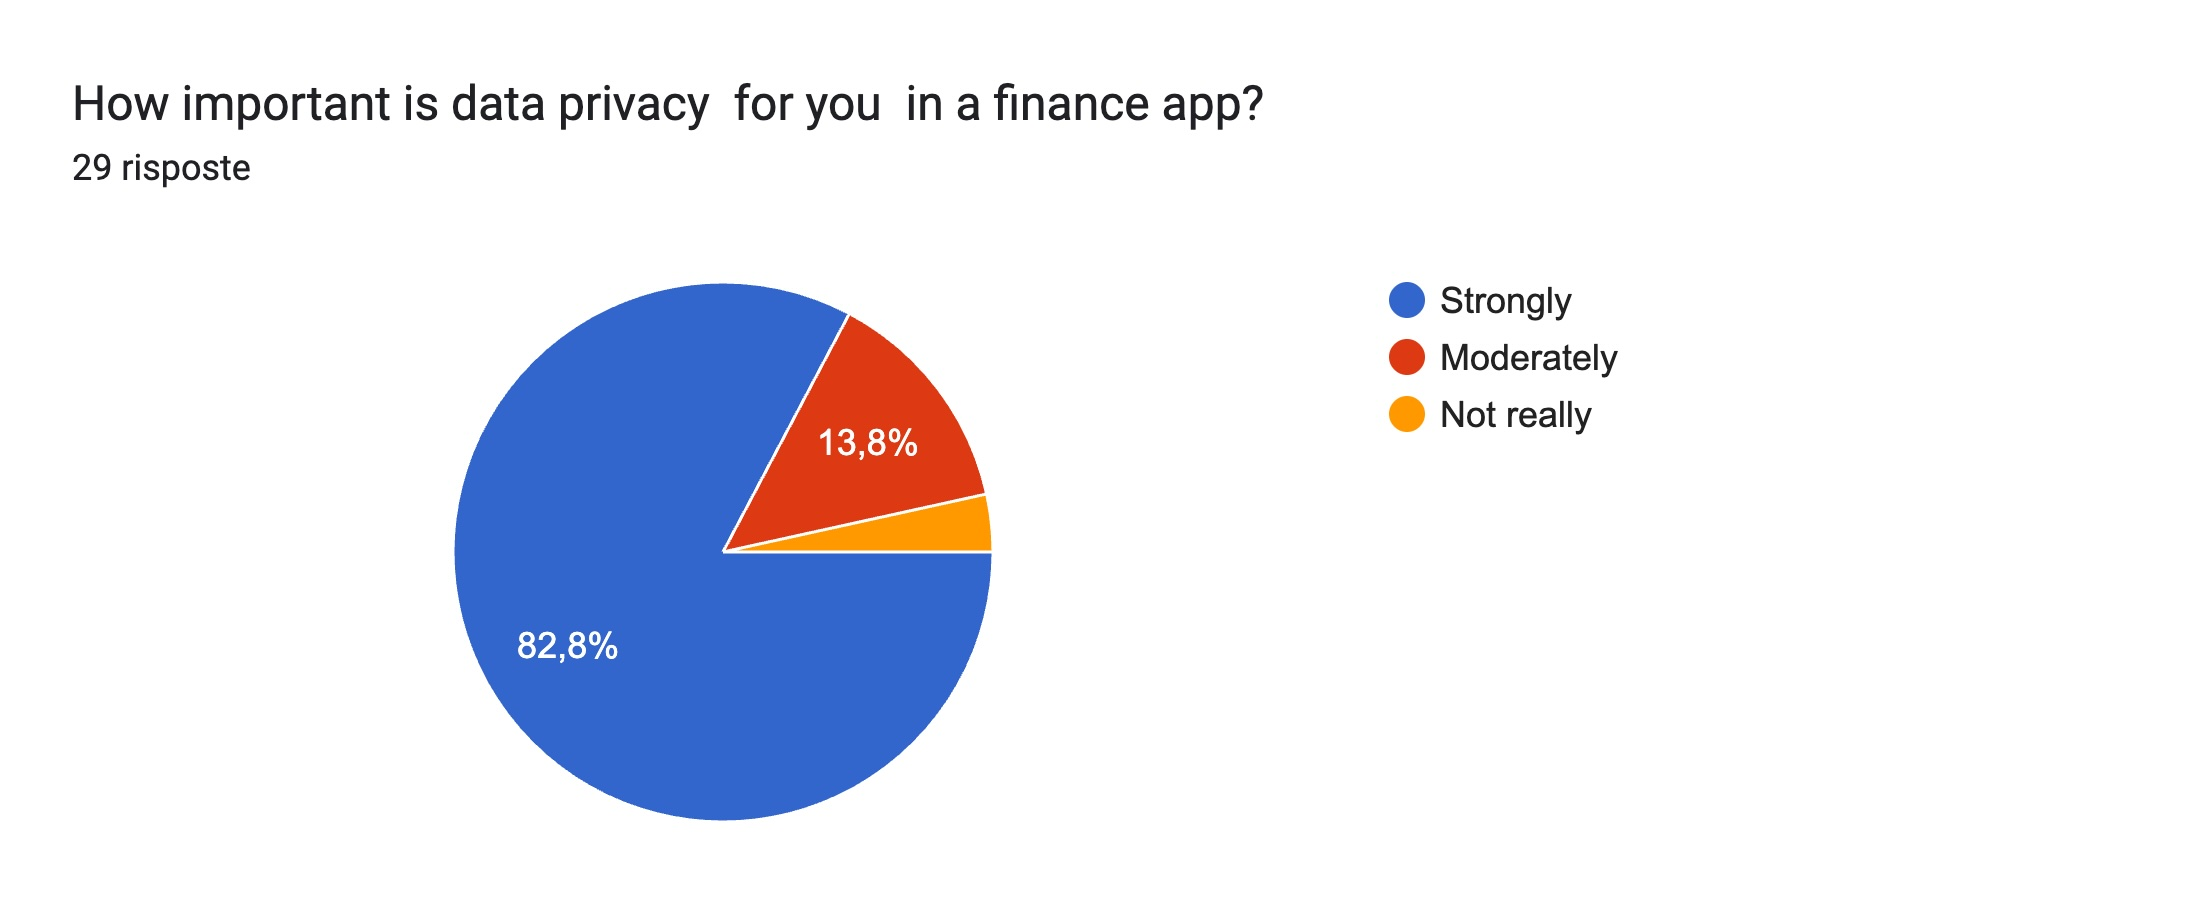
\includegraphics[width=\linewidth]{imagequest8.jpg}
\end{figure}

\subsubsection{Interview}

The feedback from the interviews with users can be synthesized into: Simplicity, Comprehensive Features, and Engaging Motivation.
\begin{itemize}
\item Simplicity and Ease of Use are Paramount
The most consistent piece of feedback, mentioned by a majority of users, is the demand for simplicity. Many current applications are perceived as "too confusing", "overcomplicated" or having a cluttered interface that resembles a spreadsheet.

\item Users want an app that is intuitive from the start, allowing for quick and easy transaction entries without filling out excessive information.
Simple graphs and charts, like pie charts showing expenses by category, are highly valued for understanding spending at a glance.
\item Many users focused on personal goals. They want to set a target (e.g., "Save €500 for a new phone"), track their progress visually, and receive encouraging notifications. The "Duolingo-style" path, where users complete small, consistent steps to reach a larger goal, was cited as a highly appealing model.
\end{itemize}
\vspace{5cm} 
\subsection{Hierarchical Task Analysis}

Hierarchical Task Analysis (HTA) is a task description methodology that is used to produce a com-
plete description of tasks in a hierarchical structure of goals, sub-goals, operations and plans in order
to have a complete representation of the action.

\subsubsection{Buy an item and record the expense}
\begin{figure}[H]
    \centering
    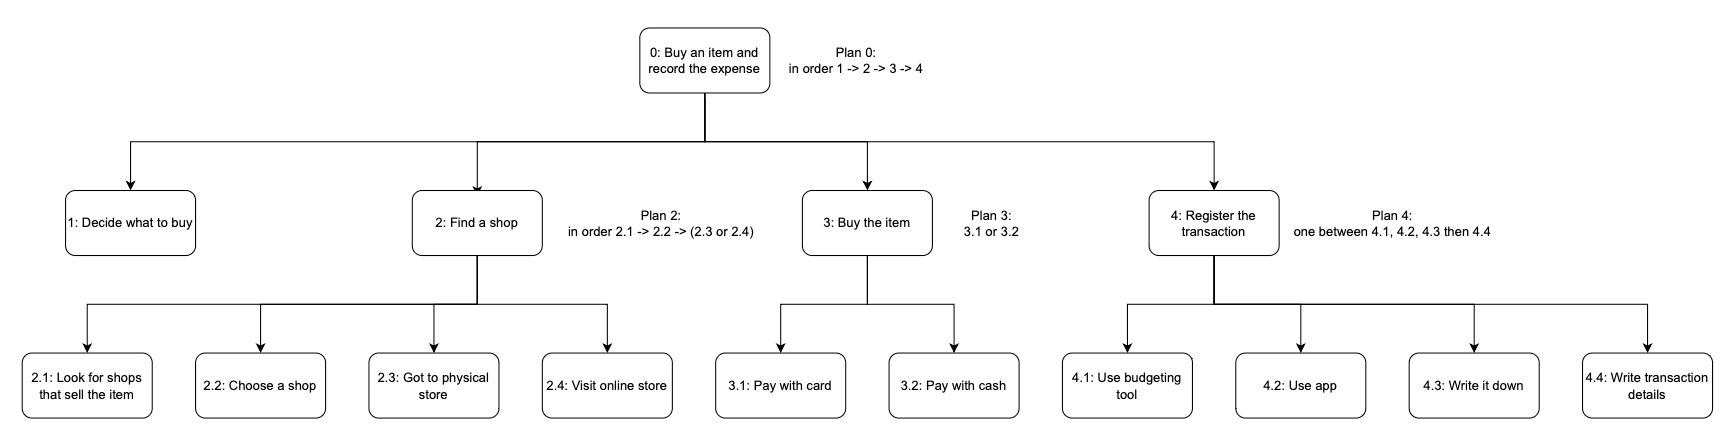
\includegraphics[width=\textwidth]{HTA1.png}
\end{figure}

\subsubsection{Set an objective and buy the related item}
\begin{figure}[H]
    \centering
    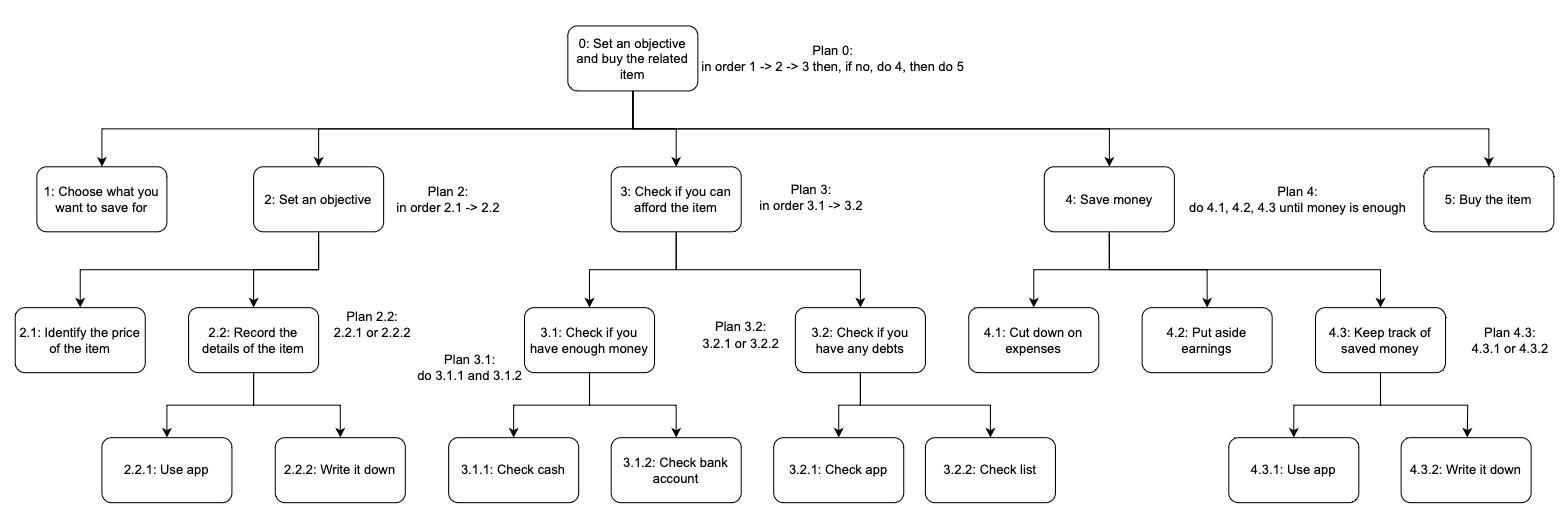
\includegraphics[width=\linewidth]{HTA2.png}
\end{figure}

\subsubsection{Extinguish a debt}
\begin{figure}[H]
    \centering
    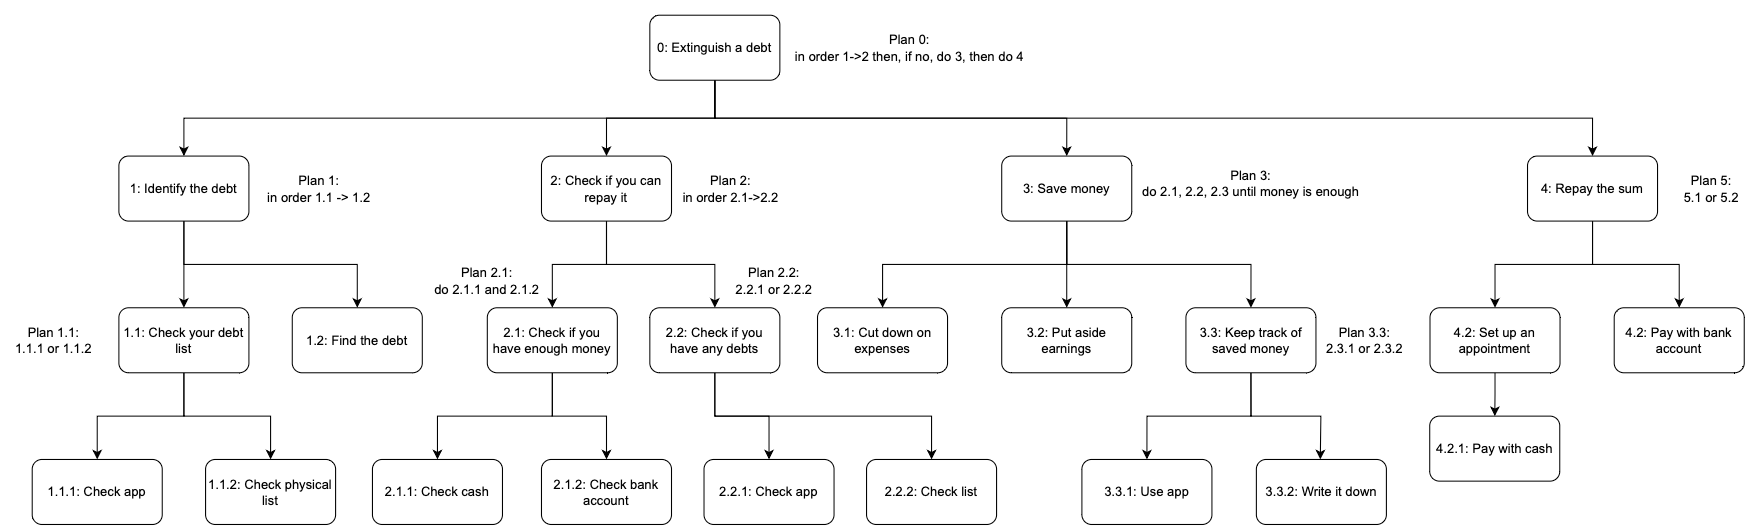
\includegraphics[width=\linewidth]{HTA3.png}
\end{figure}
\vspace{5cm} 

\subsection{Conclusions Analysis}

In conclusion, the analysis indicates a clear user need for a comprehensive and goal-oriented financial tool. The application's core functionality should be built around motivating users through Rewarding Objectives, transforming saving from a chore into an engaging challenge. To provide a complete financial picture, robust Debts and Credits handling is essential. Proactive financial planning will be enabled by a Transactions Calendar, which helps users anticipate future payments and deadlines. For insightful analysis of spending habits, the app must provide clear Percentages on kinds of purchases. Underpinning all of this is the fundamental need for user control, allowing individuals to seamlessly Create, Delete, or Change accounts, ensuring the tool remains flexible and perfectly tailored to their evolving financial lives.
\section{Design and Implementation}
State Transition Network (STN) represents a dialogue between the user and the sys-
tem, in which the system could support the tasks that the customer has to execute. It describes
which are the available actions at a certain point, and the consequent state that the system will reach.
\subsection{Add transaction}
\begin{figure}[H]
    \centering
    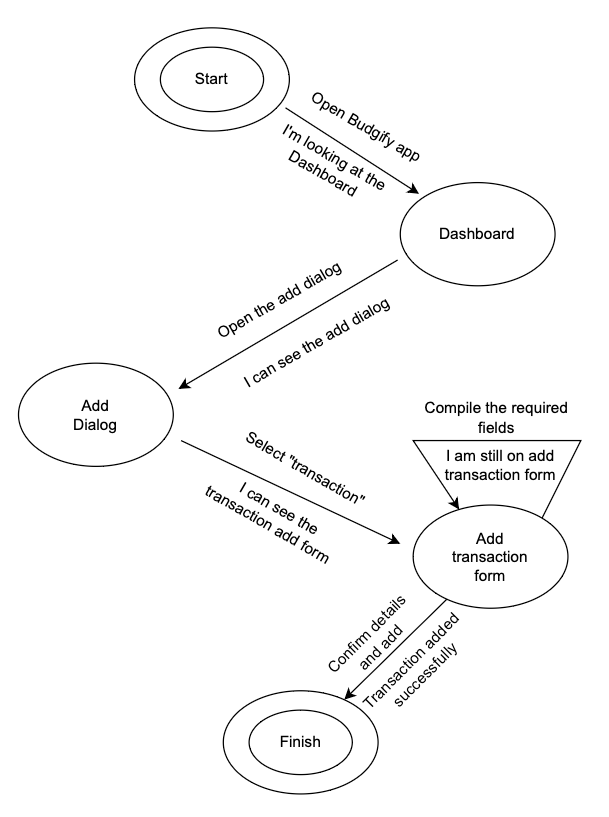
\includegraphics[scale=0.4]{STN1.png}
\end{figure}
\subsection{Set objective to buy an item}
\begin{figure}[H]
    \centering
    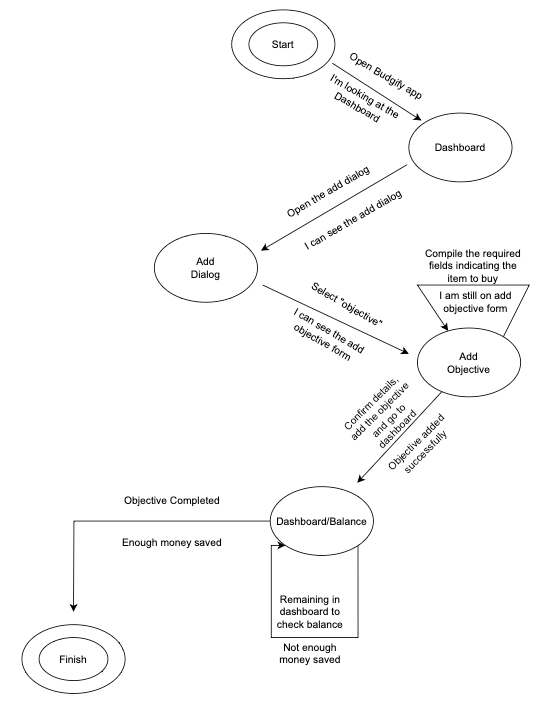
\includegraphics[scale=0.6]{STN2.png}
\end{figure}

\section{Prototype Zero}
The next focus is on creating a starting point, an initial mockup to understand how the system reacts to the intaraction with the user.
\subsection{Dashboard}
This is the landing interface of the app, the home. From here you get a sneak peak of you situation, you can see the expenses distribution from various accounts, balance and the latest transactions. From here you can navigate to other sections using the navigation bar on the bottom that is always visible.
\subsection{Transactions}
This sections allows the user to see all the transaction and with the calendar he can choose the specific day to see the transitions from that day.
\subsection{Objectives}
This is the page where the user can see the progress of his goals. We have his profile with all the statistics and by clicking the "manage objectives" button he can access the dedicated section with all the goals.
\subsection{Loans}
Here we have the Credits and Debts with a summary of both and if we click on the specific type we go to the management section.
\subsection{Categories}
In this screen we have all the categories divided by income and expense. We can manage them or adding a new one.
\subsection{Adding Section}
This is the core interaction of the app, adding "Transaction", "Objective" or "Loan". This button can be always clicked and shows the three option buttons with a pop-up.
\subsection{Settings}
Finally the settings page to chose the theme of the application, set, delete or change the pin to access the app and other informations.
\end{document}
